\documentclass{article}

\usepackage{tikz} 
\usetikzlibrary{automata, positioning, arrows} 

\usepackage{amsthm}
\usepackage{amsfonts}
\usepackage{amsmath}
\usepackage{amssymb}
\usepackage{fullpage}
\usepackage{color}
\usepackage{parskip}
\usepackage{hyperref}
\usepackage{graphicx}
\usepackage{listings}
  \hypersetup{
    colorlinks = true,
    urlcolor = blue,       % color of external links using \href
    linkcolor= blue,       % color of internal links 
    citecolor= blue,       % color of links to bibliography
    filecolor= blue,        % color of file links
    }
    
\usepackage{listings}

\lstset{escapeinside={(*@}{@*)}}

\definecolor{dkgreen}{rgb}{0,0.6,0}
\definecolor{gray}{rgb}{0.5,0.5,0.5}
\definecolor{mauve}{rgb}{0.58,0,0.82}

\lstset{frame=tb,
  language=haskell,
  aboveskip=3mm,
  belowskip=3mm,
  showstringspaces=false,
  columns=flexible,
  basicstyle={\small\ttfamily},
  numbers=none,
  numberstyle=\tiny\color{gray},
  keywordstyle=\color{blue},
  commentstyle=\color{dkgreen},
  stringstyle=\color{mauve},
  breaklines=true,
  breakatwhitespace=true,
  tabsize=3
}

\newtheoremstyle{theorem}
  {\topsep}   % ABOVESPACE
  {\topsep}   % BELOWSPACE
  {\itshape\/}  % BODYFONT
  {0pt}       % INDENT (empty value is the same as 0pt)
  {\bfseries} % HEADFONT
  {.}         % HEADPUNCT
  {5pt plus 1pt minus 1pt} % HEADSPACE
  {}          % CUSTOM-HEAD-SPEC
\theoremstyle{theorem} 
   \newtheorem{theorem}{Theorem}[section]
   \newtheorem{corollary}[theorem]{Corollary}
   \newtheorem{lemma}[theorem]{Lemma}
   \newtheorem{proposition}[theorem]{Proposition}
\theoremstyle{definition}
   \newtheorem{definition}[theorem]{Definition}
   \newtheorem{example}[theorem]{Example}
\theoremstyle{remark}    
  \newtheorem{remark}[theorem]{Remark}

\title{CPSC-354 Report}
\author{Maxwell Rovenger  \\ Chapman University}

\date{\today} 

\begin{document}

\maketitle

\begin{abstract}
% (Delete and Replace:) You can safely delete and replace the explanations in this file as they will remain available on the course website. For example, you should replace this abstract with your own. The abstract should be a short summary of the report. It should be written in a way that makes it possible to understand the purpose of the report without reading it.  
\end{abstract}

\setcounter{tocdepth}{3}
\tableofcontents

\section{Introduction}\label{intro}

(Delete and Replace): This report will document your learning throughout the course. It will be a collection of your notes, homework solutions, and critical reflections on the content of the course. Something in between a semester-long take home exam and your own lecture notes.\footnote{One purpose of giving the report the form of lecture notes is that self-explanation is a technique proven to help with learning, see Chapter 6 of Craig Barton, How I Wish I'd Taught Maths, and references therein. In fact, the report can lead you from self-explanation (which is what you do for the weekly deadline) to explaining to others (which is what you do for the final submission). Another purpose is to help those of you who want to go on to graduate school to develop some basic writing skills. A report that you could proudly add to your application to graduate school (or a job application in industry) would give you full points.}

To modify this template you need to modify the source \texttt{report.tex} which is available in the course repo. For guidance on how to do this read both the source and the pdf of \texttt{latex-example.tex} which is also available in the repo. Also check out the usual resources (Google, Stackoverflow, LLM, etc). It was never as easy as now to learn a new programming lanugage (which, btw, \LaTeX{} is).

For writing \LaTeX{} with VSCode use the \href{https://marketplace.visualstudio.com/items?itemName=James-Yu.latex-workshop}{LaTeX Workshop} extension. 

There will be deadlines during the semester, graded mostly for completeness. That means that you will get the points if you submit in time and are on the right track, independently of whether the solutions are technically correct. You will have the opportunity to revise your work for the final submission of the full report.

The full report is due at the end of the finals week. It will be graded according to the following guidelines.

\section{Week by Week}\label{homework}

\subsection{Week 1}

\subsubsection*{Notes}

Lectures introduced Lean, a programming language to help prove discrete mathematics proofs. Through using the Natural Numbers Game, we saw how Lean operates and how it works it can, with functions acting as steps, prove theorems similar to how we did in discrete math with pen and paper and induction.

\subsubsection*{Homework}

Solved problems in Natural Numbers Game using Lean to help recap teachings from Discrete Mathematics. Specifically dealing with successors and predecessors and how they can be used to change certain sides to equal the other.

Level 5/8:
\begin{lstlisting}
a + (b + 0) + (c + 0) = a + b + c
rw [add_zero]
a + b + (c + 0) = a + b + c
rw [add_zero]
a + b + c = a + b + c
rfl
\end{lstlisting}

Level 6/8:
\begin{lstlisting}
a + (b + 0) + (c + 0) = a + b + c
rw[add_zero c]
a + (b + 0) + c = a + b + c
rw[add_zero b]
a + b + c = a + b + c
rfl
\end{lstlisting}

Level 7/8:
\begin{lstlisting}
succ n = n + 1
rw[one_eq_succ_zero]
succ n = n + succ 0
rw[add_succ]
succ n = succ (n + 0)
rw[add_zero]
succ n = succ n
rfl
\end{lstlisting}

Level 8/8:
\begin{lstlisting}
2 + 2 = 4
rw[four_eq_succ_three]
2 + 2 = succ 3
rw[three_eq_succ_two]
2 + 2 = succ (succ 2)
rw[two_eq_succ_one]
succ 1 + succ 1 = succ (succ (succ 1))
rw[add_succ]
succ (succ 1 + 1) = succ (succ (succ 1))
rw[succ_eq_add_one]
succ 1 + 1 + 1 = succ (succ (succ 1))
rw[succ_eq_add_one]
1 + 1 + 1 + 1 = succ (succ (1 + 1))
rw[succ_eq_add_one]
1 + 1 + 1 + 1 = succ (1 + 1) + 1
rw[succ_eq_add_one]
1 + 1 + 1 + 1 = 1 + 1 + 1 + 1
rfl
\end{lstlisting}

For level 5/8 specifically, we can see that the Lean proof, \texttt{rw[add\_zero]}, corresponds to Proof Algorithm 1: Addition, in that any variable added to zero will ultimately equal just the variable. For example: $a + 0 = a$.

From this homework, I learned how to use the Lean proof and saw how each function operated exactly like algorithms and proofs I had used in Discrete Mathematics.

%In case you want to draw automata in Latex, you can use the tikz %package. Here is an example of a simple automaton:
%
%\begin{tikzpicture}[shorten >=1pt,node distance=2cm,on grid,auto] 
%  \node[state] (q_1)   {$q_1$}; 
%  \node[state] (q_2) [above right=of q_1] {$q_2$}; 
%  \node[state] (q_3) [below right=of q_2] {$q_3$}; 
%   \path[->] 
%   (q_1) edge  node {0} (q_2)
%         edge  node [swap] {1} (q_3)
%   (q_2) edge  node  {1} (q_3)
%         edge [loop above] node {0} ()
%   (q_3) edge [loop below] node {0,1} ();
%\end{tikzpicture}
%
%By the way, GPT-4 is quite good at outputting tikz code.

\subsubsection*{Comments and Questions}

Although this week generally served as just an introduction to the curriculum and a recap of discrete mathematics, I am curious as to whether or not there was a better example to be shown of how exactly a computer uses discrete mathematics. At this point, I am knowledgeable of how discrete mathematics operates and how computers can use operators to conduct mathematical operations, but I have yet to see a direct example of a computer "thinking" through a math calculation.

If the way computers have been taught mathematics is based purely on successors and predecessors, does that make other operations like multiplication, division, and exponents far more taxing on a CPU since they have to calculate an incredible amount of successors, or do the operators used to cause multiplication and exponentiation ignore that by just creating duplicates and adding them together?

%I expect you to read the lecture notes. 

\subsection{Week 2}

\subsubsection*{Notes}

Recursion, in coding, allows for more simplistic code that is easier to read, scale, and apply. 

Regarding the allowing of typos in coding, code should be non-ambigious because coding should be universal and should work the same within the same virtual machine regardless of how you access it. We see examples of this in GitHub's copilot since it only makes suggestions that are non-ambigious and can work on any machine, as long as they have the correct virtual machine.

Lean contains tactics, Ex: rw, and theorems, Ex: one\_eq\_succ\_zero. Tactics are commands while theorems are logical propositions.

\subsubsection*{Homework}
Level 1/5:
\begin{lstlisting}
0 + n = n
induction n with d hd
0 + 0 = 0
rw[add_zero]
0 = 0
rfl
0 + succ d = succ d
rw[add_succ]
succ (0 + d) = succ d
rw[hd]
succ d = succ d
rfl
\end{lstlisting}

Level 2/5:
\begin{lstlisting}
succ a + b = succ (a + b)
induction b with b
succ a + 0 = succ (a + 0)
rw[add_zero]
succ a = succ (a + 0)
rw[add_zero]
succ a = succ a
rfl
succ a + succ b = succ (a + succ b)
rw[add_succ]
succ (succ a + b) = succ (a + succ b)
rw[n_ih]
succ (succ (a + b)) = succ (a + succ b)
rw[add_succ]
succ (succ (a + b)) = succ (succ (a + b))
rfl
\end{lstlisting}

Level 3/5:
\begin{lstlisting}
a + b = b + a
induction b with b hb
a + 0 = 0 + a
rw [add_zero]
a = 0 + a
rw [zero_add]
a = a
rfl
a + succ b = succ b + a
rw [add_succ]
succ (a + b) = succ b + a
rw [hb]
succ (b + a) = succ b + a
rw [succ_add]
succ (b + a) = succ (b + a)
rfl
\end{lstlisting}

Level 4/5:
\begin{lstlisting}
a + b + c = a + (b + c)
induction c with c hc
a + b + 0 = a + (b + 0)
rw [add_zero]
a + b = a + (b + 0)
rw [add_zero]
a + b = a + b
rfl
a + b + succ c = a + (b + succ c)
rw [add_succ]
succ (a + b + c) = a + (b + succ c)
rw [add_succ]
succ (a + b + c) = a + succ (b + c)
rw [add_succ]
succ (a + b + c) = succ (a + (b + c))
rw [hc]
succ (a + (b + c)) = succ (a + (b + c))
rfl
\end{lstlisting}

Level 5/5:
\begin{lstlisting}
a + b + c = a + c + b
induction c with c hc
a + b + 0 = a + 0 + b
rw [add_zero, add_zero]
a + b = a + b
rfl
a + b + succ c = a + succ c + b
rw [add_succ]
succ (a + b + c) = a + succ c + b
rw [add_succ]
succ (a + b + c) = succ (a + c) + b
rw [succ_add]
succ (a + b + c) = succ (a + c + b)
rw [hc]
succ (a + c + b) = succ (a + c + b)
rfl
\end{lstlisting}
\subsubsection*{Comments and Questions}

Personally, I felt that when it comes to AI autocorrecting code, instead of being lenient towards mistyped code, AI could just simply correct the typos. This would allow for a smoother coding process wihle also creating non-ambigious code.

After playing around with the Tower of Hanoi, it is apparent that recursion is invaluable in programming. We often see it as a way to neatly write code but it can also be massive time saver as apparent with the Tower of Hanoi where instead of having to, through trial and error finding out the solution, we can just use a recursive equation and plug in our values. My question then is, in what other fields can we apply recursion, as it is becoming more apparent to me that recursion can be a form of thinking rather than a field specific method?

\subsubsection*{Lean Proof}

\begin{align*}
  a + b + c = a + (b + c) \\
  a + b + 0 = a + (b + 0) == def of + \\
  a + b = a + (b + 0) == def of + \\
  a + b = a + b \\
\end{align*}

\subsection{Week 3}

\subsubsection*{Notes}

It is impossible for a computer to prove all mathematical proofs since there are statements in arithmetic that are unclear if they are true or not and thus cannot be proved. This is due to there being proofs in mathematics that are built based upon assumption and although there are no problems found so far, they cannot be proved through ordinary means like what the computer would opt to do.

\subsubsection*{Homework}

\href{https://github.com/mrovengerdev/LLM-literature-review/blob/main/README.md}{LLM Literature Review README}

\subsubsection*{Discord Posting}

For my literature review, I used ChatGPT4 to ask questions about recursion within computer systems. More specifically, if it decreases memory usage or provides any processing speed based benefits rather than just readability or integration based benefits. Through my conversation, I learned that due to creating more and more stack frames for each iteration, recursion can actually increase memory usage. However, there is an alternative, that being tail recursion. It was developed in 1970s however it either does not have support or only has limited support for popular languages like Python and JavaScript. Thus, it was concluded that recursive functions are actually less memory efficient than iterative solutions. This surprised me as through recursion, humans are able to abstract a lot of our thinking and are able to quickly find out what the next iterative output is. This contrasts computers which require more processing power to perform recursive methods. This creates an inverse relationship where the better the human understanding, the worse the computer understanding.

\subsection{Week 4}

\subsubsection*{Notes}

An abstract syntax tree is the result of parsing and helps display the order and relationship between operators in a mathematical problem. the abstract syntax tree is the most intermediate, as it is more drawn out than both concrete syntax and a concrete syntax tree.

We can define well formed expressions through formal grammar. Since formal grammar helps to create definitions for what becomes a well-formed expression.

\subsubsection*{Homework}

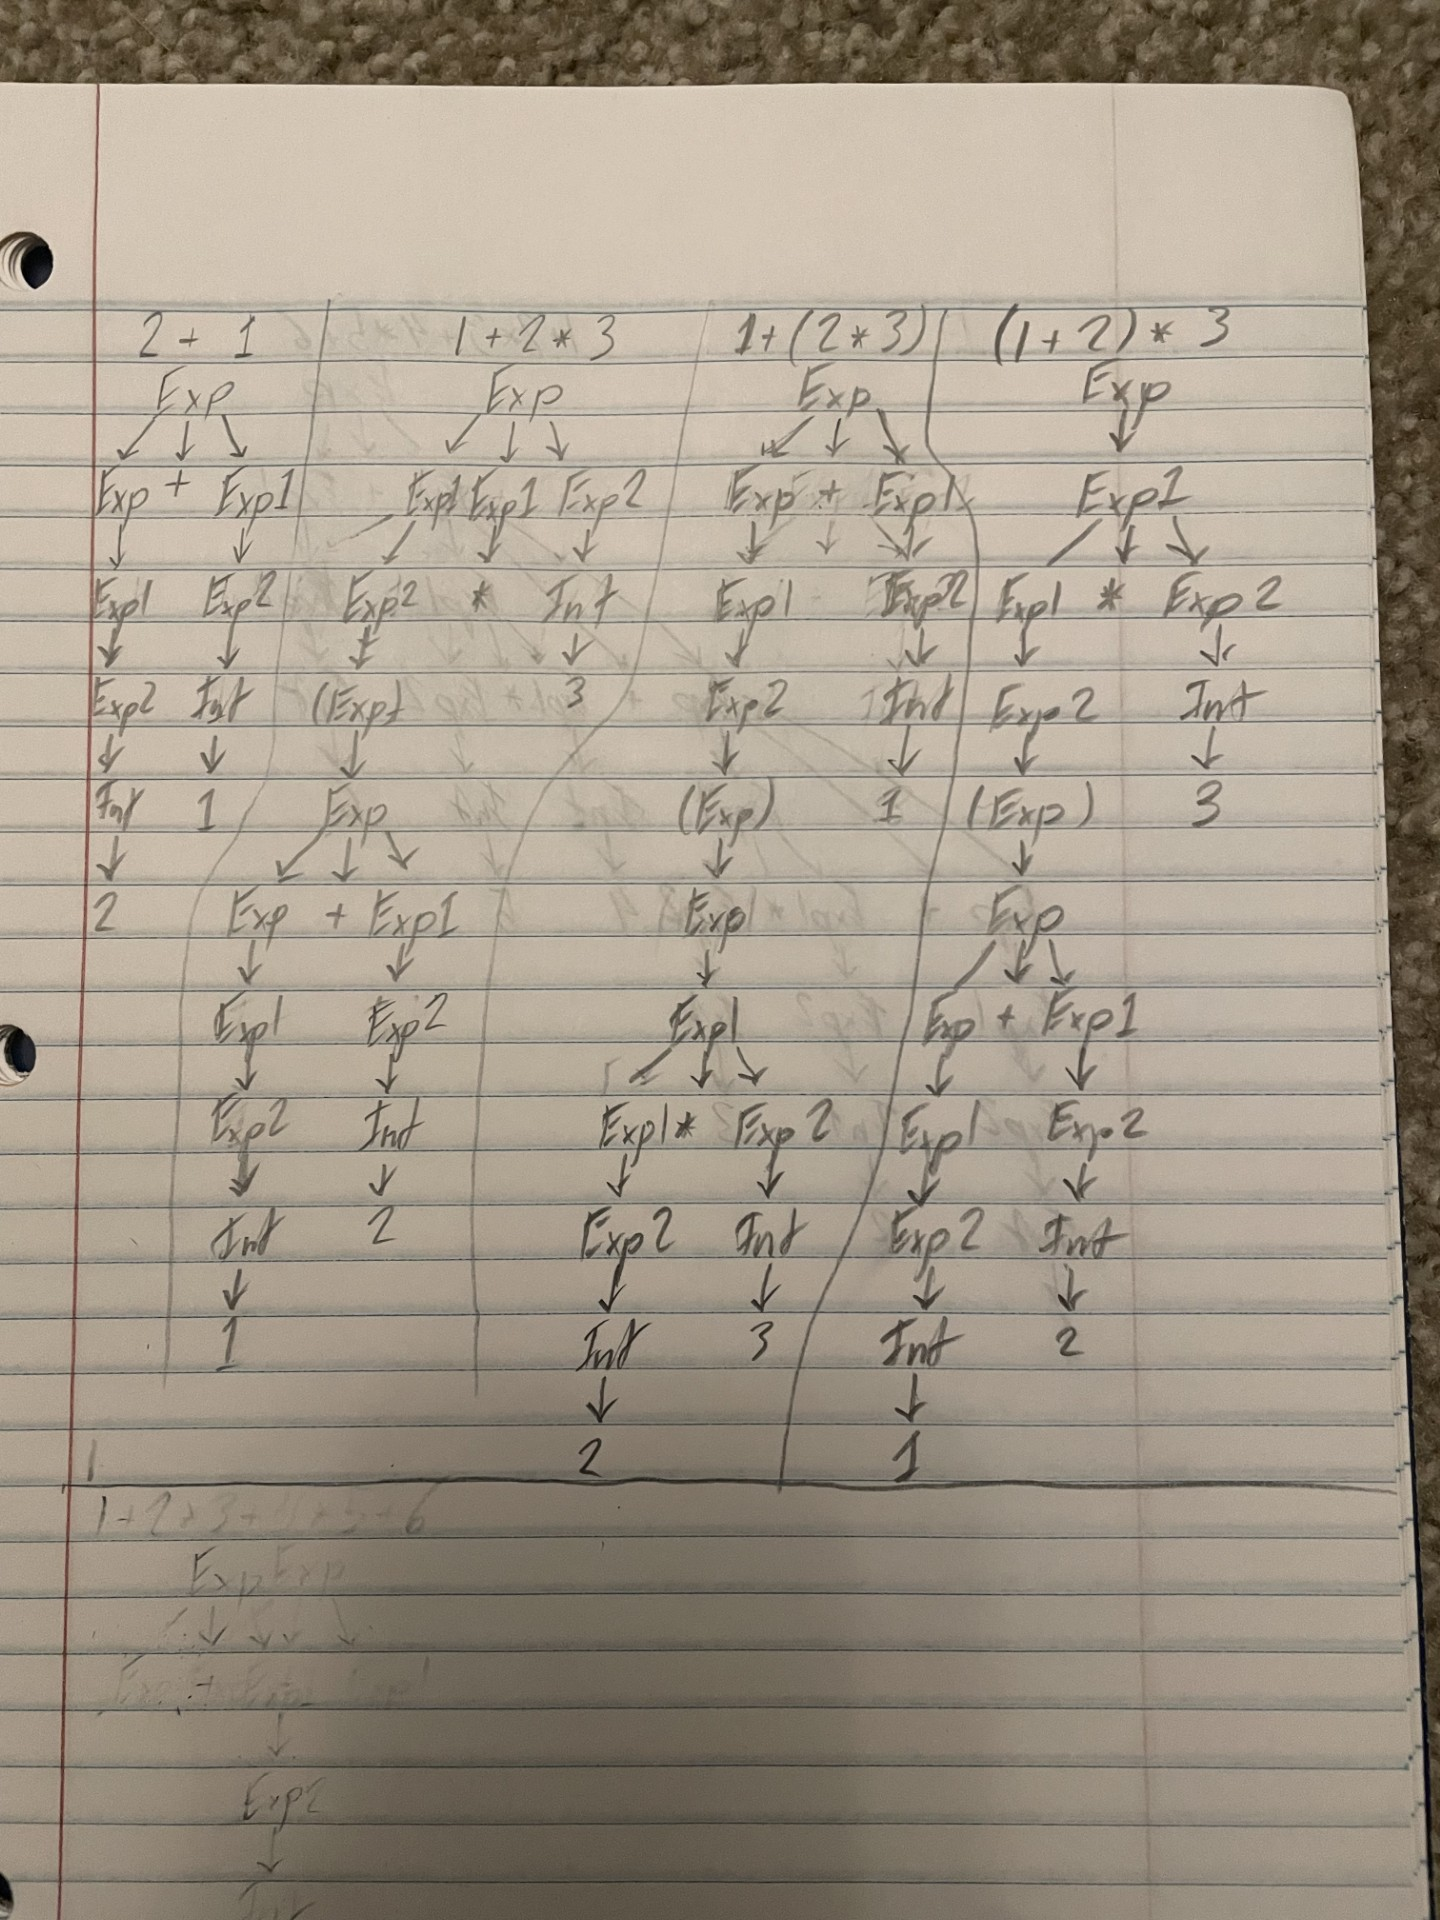
\includegraphics[width=0.45\textwidth]{HW4IMG1.jpg}
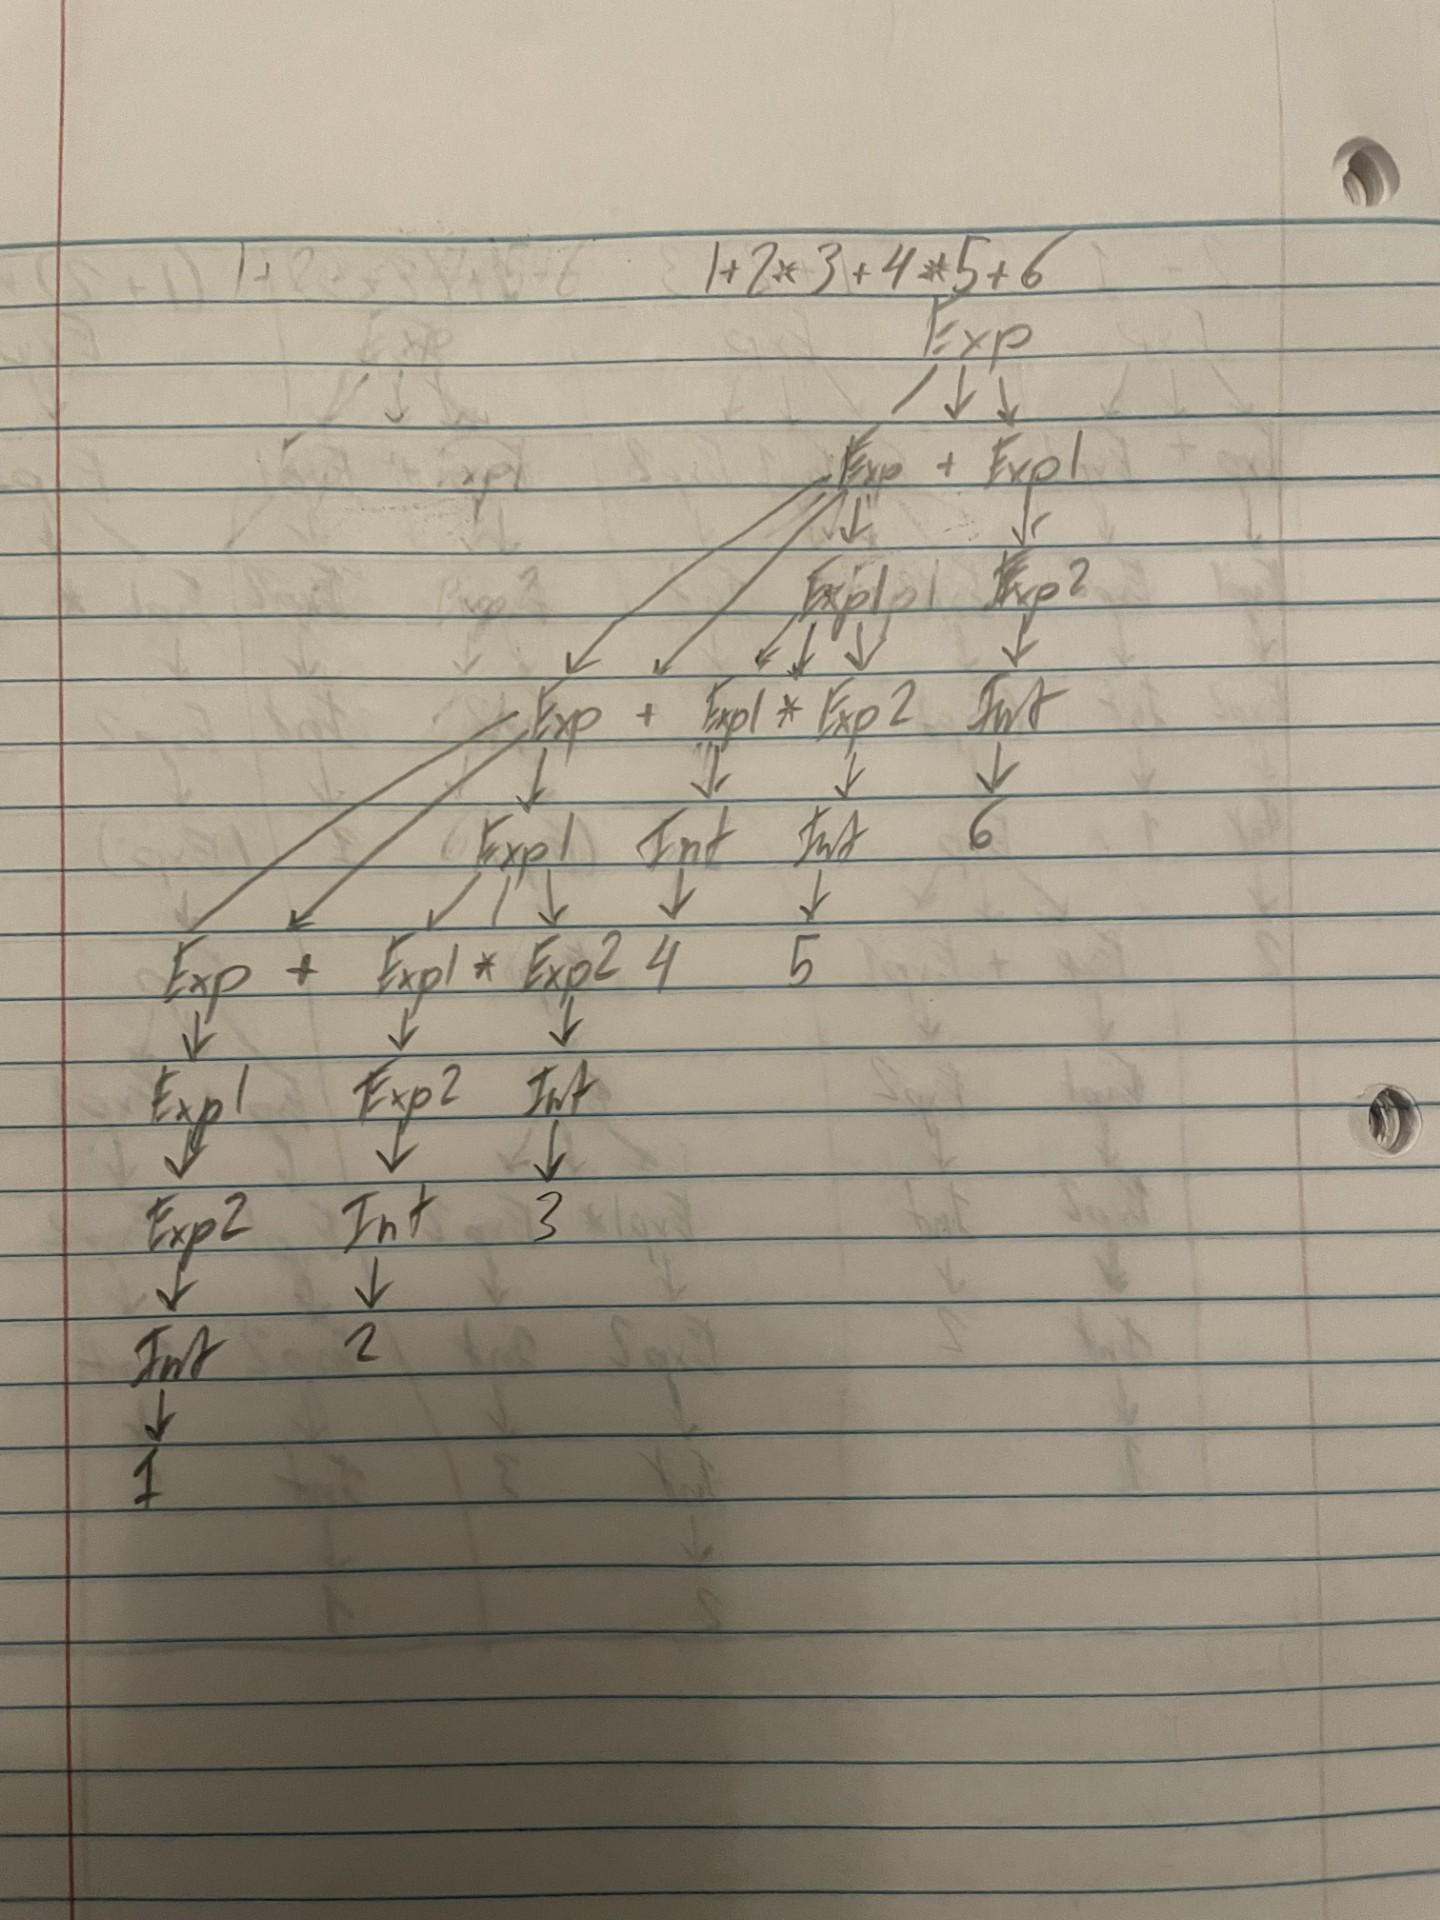
\includegraphics[width=0.45\textwidth]{HW4IMG2.jpg}

\subsubsection*{Questions and Comments}

If my understanding is correct, all formal languages are allowed to have their own alphabets and grammar that must be defined. However, we have found ourselves in a position where the majority of, if not all, programming langauges will use the same characters or symbols for operators and values. Thus, my question is if there is a protocol enforced that mandates the formal language used in a programming languages or has this all occurred just for ease of use?

\subsection{Week 5}

\subsubsection*{Notes}

In this week's lecture, we learned about the logic behind AND and how computer's process it. This shows that a proof in logic can be represented as a program in a programming language and vice versa.

Similarly, in the natural numbers game, we saw the application of these theorems which allowed us to prove theorems in Lean. So if a refresher is needed, going through the "A Lean Intro To Logic" is a good idea.

\subsubsection*{Homework}
Level 1/8:
\begin{lstlisting}
todo_list: P
exact todo_list
\end{lstlisting}

Level 2/8:
\begin{lstlisting}
(*@ $[ Goal: P \land S ]$ @*)
exact and_intro p s
\end{lstlisting}

Level 3/8:
\begin{lstlisting}
(*@ $[ Goal: (A \land I) \land O \land U ]$ @*)
exact and_intro (and_intro a i) (and_intro o u)
\end{lstlisting}

Level 4/8:
\begin{lstlisting}
Assumptions:
  (*@ $[ - vm: P \land S ]$ @*)
have p := vm.left
Assumptions: 
  (*@ $[ - vm: P \land S ]$ @*)
  (*@ $[ - p: P ]$ @*)
exact p
\end{lstlisting}

Level 5/8:
\begin{lstlisting}
Assumptions:
  (*@ $[ - h: P \land Q ]$ @*)
have q := and_right h
Assumptions:
  (*@ $[ - h: P \land Q ]$ @*)
  (*@ $[ - q: Q ]$ @*)
exact q
\end{lstlisting}

Level 6/8:
\begin{lstlisting}
Assumptions:
  (*@ $[ - h1: A \land I ]$ @*)
  (*@ $[ - h2: O \land U ]$ @*)
have A := and_left h1
Assumptions:
  (*@ $[ - h1: A \land I ]$ @*)
  (*@ $[ - h2: O \land U ]$ @*)
  (*@ $[ - A: A ]$ @*)
have U := and_right h2
Assumptions:
  (*@ $[ - h1: A \land I ]$ @*)
  (*@ $[ - h2: O \land U ]$ @*)
  (*@ $[ - A: A ]$ @*)
  (*@ $[ - U: U ]$ @*)
exact and_intro A U
\end{lstlisting}

Level 7/8:
\begin{lstlisting}
Assumptions:
  (*@ $[ - h: (L \land ((L \land C) \land L) \land L \land L \land L) \land (L \land L) \land L ]$ @*)
have h1 := and_left h
Assumptions:
  (*@ $[ - h: (L \land ((L \land C) \land L) \land L \land L \land L) \land (L \land L) \land L ]$ @*)
  (*@ $[ - h1: L \land ((L \land C) \land L) \land L \land L \land L ]$ @*)
have h2 := and_right h1
Assumptions:
  (*@ $[ - h: (L \land ((L \land C) \land L) \land L \land L \land L) \land (L \land L) \land L ]$ @*)
  (*@ $[ - h1: L \land ((L \land C) \land L) \land L \land L \land L ]$ @*)
  (*@ $[ - h2: ((L \land C) \land L) \land L \land L \land L ]$ @*)
have h3 := and_left h2
Assumptions:
  (*@ $[ - h: (L \land ((L \land C) \land L) \land L \land L \land L) \land (L \land L) \land L ]$ @*)
  (*@ $[ - h1: L \land ((L \land C) \land L) \land L \land L \land L ]$ @*)
  (*@ $[ - h2: ((L \land C) \land L) \land L \land L \land L ]$ @*)
  (*@ $[ - h3: (L \land C) \land L ]$ @*)
have h4 := and_left h3
Assumptions:
  (*@ $[ - h: (L \land ((L \land C) \land L) \land L \land L \land L) \land (L \land L) \land L ]$ @*)
  (*@ $[ - h1: L \land ((L \land C) \land L) \land L \land L \land L ]$ @*)
  (*@ $[ - h2: ((L \land C) \land L) \land L \land L \land L ]$ @*)
  (*@ $[ - h3: (L \land C) \land L ]$ @*)
  (*@ $[ - h4: L \land C ]$ @*)
have h5 := and_right h4
Assumptions:
  (*@ $[ - h: (L \land ((L \land C) \land L) \land L \land L \land L) \land (L \land L) \land L ]$ @*)
  (*@ $[ - h1: L \land ((L \land C) \land L) \land L \land L \land L ]$ @*)
  (*@ $[ - h2: ((L \land C) \land L) \land L \land L \land L ]$ @*)
  (*@ $[ - h3: (L \land C) \land L ]$ @*)
  (*@ $[ - h4: L \land C ]$ @*)
  (*@ $[ - h5: C ]$ @*)
exact h5
\end{lstlisting}

Level 8/8:
\begin{lstlisting}
Assumptions:
  (*@ $[ - h: ((P \land S) \land A) \land \neg I \land (C \land \neg O) \land \neg U ]$ @*) and_left (1)
have h1 := and_left h
Assumptions:
  (*@ $[ - h: ((P \land S) \land A) \land \neg I \land (C \land \neg O) \land \neg U ]$ @*)
  (*@ $[ - h1: (P \land S) \land A ]$ @*)
have h2 := and_left h1
Assumptions:
  (*@ $[ - h: ((P \land S) \land A) \land \neg I \land (C \land \neg O) \land \neg U ]$ @*)
  (*@ $[ - h1: (P \land S) \land A ]$ @*)
  (*@ $[ - h2: P \land S ]$ @*)
have h3 := and_right h1
Assumptions:
  (*@ $[ - h: ((P \land S) \land A) \land \neg I \land (C \land \neg O) \land \neg U ]$ @*)
  (*@ $[ - h1: (P \land S) \land A ]$ @*)
  (*@ $[ - h2: P \land S ]$ @*)
  (*@ $[ - h3: A ]$ @*)
have h4 := and_right h
Assumptions:
  (*@ $[ - h: ((P \land S) \land A) \land \neg I \land (C \land \neg O) \land \neg U ]$ @*)
  (*@ $[ - h1: (P \land S) \land A ]$ @*)
  (*@ $[ - h2: P \land S ]$ @*)
  (*@ $[ - h3: A ]$ @*)
  (*@ $[ - h4: \neg I \land (C \land \neg O) \land \neg U ]$ @*)
have h5 := and_right h4
Assumptions:
  (*@ $[ - h: ((P \land S) \land A) \land \neg I \land (C \land \neg O) \land \neg U ]$ @*)
  (*@ $[ - h1: (P \land S) \land A ]$ @*)
  (*@ $[ - h2: P \land S ]$ @*)
  (*@ $[ - h3: A ]$ @*)
  (*@ $[ - h4: \neg I \land (C \land \neg O) \land \neg U ]$ @*)
  (*@ $[ - h5: (C \land \neg O) \land \neg U ]$ @*)
have h6 := and_left h5
Assumptions:
  (*@ $[ - h: ((P \land S) \land A) \land \neg I \land (C \land \neg O) \land \neg U ]$ @*)
  (*@ $[ - h1: (P \land S) \land A ]$ @*)
  (*@ $[ - h2: P \land S ]$ @*)
  (*@ $[ - h3: A ]$ @*)
  (*@ $[ - h4: \neg I \land (C \land \neg O) \land \neg U ]$ @*)
  (*@ $[ - h5: (C \land \neg O) \land \neg U ]$ @*)
  (*@ $[ - h6: C \land \neg O ]$ @*)
have h7 := and_left h6
Assumptions:
  (*@ $[ - h: ((P \land S) \land A) \land \neg I \land (C \land \neg O) \land \neg U ]$ @*)
  (*@ $[ - h1: (P \land S) \land A ]$ @*)
  (*@ $[ - h2: P \land S ]$ @*)
  (*@ $[ - h3: A ]$ @*)
  (*@ $[ - h4: \neg I \land (C \land \neg O) \land \neg U ]$ @*)
  (*@ $[ - h5: (C \land \neg O) \land \neg U ]$ @*)
  (*@ $[ - h6: C \land \neg O ]$ @*)
  (*@ $[ - h7: C ]$ @*)
have h8 := and_left h2
Assumptions:
  (*@ $[ - h: ((P \land S) \land A) \land \neg I \land (C \land \neg O) \land \neg U ]$ @*)
  (*@ $[ - h1: (P \land S) \land A ]$ @*)
  (*@ $[ - h2: P \land S ]$ @*)
  (*@ $[ - h3: A ]$ @*)
  (*@ $[ - h4: \neg I \land (C \land \neg O) \land \neg U ]$ @*)
  (*@ $[ - h5: (C \land \neg O) \land \neg U ]$ @*)
  (*@ $[ - h6: C \land \neg O ]$ @*)
  (*@ $[ - h7: C ]$ @*)
  (*@ $[ - h8: P ]$ @*)
have h9 := and_right h2
Assumptions:
  (*@ $[ - h: ((P \land S) \land A) \land \neg I \land (C \land \neg O) \land \neg U ]$ @*)
  (*@ $[ - h1: (P \land S) \land A ]$ @*) 
  (*@ $[ - h2: P \land S ]$ @*) 
  (*@ $[ - h3: A ]$ @*) 
  (*@ $[ - h4: \neg I \land (C \land \neg O) \land \neg U ]$ @*) 
  (*@ $[ - h5: (C \land \neg O) \land \neg U ]$ @*) 
  (*@ $[ - h6: C \land \neg O ]$ @*) 
  (*@ $[ - h7: C ]$ @*)
  (*@ $[ - h8: P ]$ @*)
  (*@ $[ - h9: S ]$ @*)
exact and_intro h3 (and_intro h7 (and_intro h8 h9))
\end{lstlisting}

level 8/8 in Mathematical Logic
\[
\begin{aligned}
    (1) &\quad ((P \land S) \land A) \land \neg I \land (C \land \neg O) \land \neg U & \text{assumption} \\
    (2) &\quad (P \land S) \land A & \text{and\_left (1)} \\
    (3) &\quad P \land S & \text{and\_left (2)} \\
    (4) &\quad A & \text{and\_right (2)} \\
    (5) &\quad \neg I \land (C \land \neg O) \land \neg U & \text{and\_right (1)} \\
    (6) &\quad (C \land \neg O) \land \neg U & \text{and\_right (5)} \\
    (7) &\quad C \land \neg O & \text{and\_left (6)} \\
    (8) &\quad C & \text{and\_left (7)} \\
    (9) &\quad P & \text{and\_left (3)} \\
    (10) &\quad S & \text{and\_right (3)} \\
\end{aligned}
\]

\subsubsection*{Comments and Questions}

Following our exposure to proving the new theorem regarding "AND" in Lean, I took note of the recursive nature of this course. Specifically, how all topics in this course build up on each other. This lead me to asking the question: How does recursion play into isomorphism and is the scalability of recursive functions a necessity for theorems and logic within programming?

\section{Lessons from the Assignments}

(Delete and Replace): Write three pages about your individual contributions to the project.

On 3 pages you describe lessons you learned from the project. Be as technical and detailed as possible. Particularly valuable are \emph{interesting} examples where you connect concrete technical details with \emph{interesting} general observations or where the theory discussed in the lectures helped with the design or implementation of the project.

Write this section during the semester. This is approximately a quarter of apage per week and the material should come from the work you do anyway. Just keep your eyes open for interesting lessons.

Make sure that you use \LaTeX{} to structure your writing (eg by using subsections).

\section{Conclusion}\label{conclusion}

(Delete and Replace): (approx 400 words) A critical reflection on the content of the course. Step back from the technical details. How does the course fit into the wider world of software engineering? What did you find most interesting or useful? What improvements would you suggest?

\begin{thebibliography}{99}
\bibitem[BLA]{bla} Author, \href{https://en.wikipedia.org/wiki/LaTeX}{Title}, Publisher, Year.
\end{thebibliography}

\end{document}
